\documentclass[10pt]{beamer}
\usepackage[utf8]{inputenc}
\usepackage[czech]{babel}
\usepackage[abs]{overpic}
\usepackage{color}
\usepackage{tikz}

\usepackage[normalem]{ulem}
\usepackage{soul}

\newcommand{\tabitem}{~~\llap{\textbullet}~~}

\newcommand{\myurl}[1]{\href{#1}{\color{blue}{\url{#1}}}}

\definecolor{myred}{HTML}{D26966}
\definecolor{myblue}{HTML}{578CC2}

\usetheme[faculty=fi]{fibeamer}

\title[Formal Analysis of Rule-Based
Models in Systems Biology]{Formal Analysis of Rule-Based
Models\\ in Systems Biology}
\subtitle{Thesis proposal defense}

\date{\today}
\author[Matej Troj\'{a}k]{ Matej Troj\'{a}k}

\setbeamertemplate{footline}
{
  \leavevmode
  \hbox{
  \begin{beamercolorbox}[wd=.15\paperwidth,ht=2.25ex,dp=1ex,center]{title in head/foot}
    \usebeamerfont{author in head/foot}\insertshortauthor
  \end{beamercolorbox}

  \begin{beamercolorbox}[wd=.7\paperwidth,ht=2.25ex,dp=1ex,center]{author in head/foot}
    \usebeamerfont{author in head/foot}\insertshorttitle
  \end{beamercolorbox}

  \begin{beamercolorbox}[wd=.15\paperwidth,ht=2.25ex,dp=1ex,center]{title in head/foot}
    \insertframenumber{} / \inserttotalframenumber
  \end{beamercolorbox}
  }
}

\AtBeginSection[]
{
  \begin{frame}<beamer>
    \tableofcontents[currentsection]
  \end{frame}
}

\newcommand{\backupbegin}{
   \newcounter{framenumberappendix}
   \setcounter{framenumberappendix}{\value{framenumber}}
}
\newcommand{\backupend}{
   \addtocounter{framenumberappendix}{-\value{framenumber}}
   \addtocounter{framenumber}{\value{framenumberappendix}} 
}

\begin{document}

\thispagestyle{empty}
\maketitle

% --------------------------------------------------------

\begin{frame}[fragile]{Motivation}

\begin{minipage}{0.55\textwidth}
\begin{itemize}
	\item We have some \textbf{questions} about a (\emph{biological}) system which need to be answered.
\end{itemize}
\end{minipage}
\hfill
\begin{minipage}{0.44\textwidth}
\begin{center}

\includegraphics[scale=0.15]{pics/bacteria.png}
\end{center}
\end{minipage}


\begin{minipage}{0.33\textwidth}
\begin{center}

\includegraphics[scale=0.1]{pics/pipette.png}
\end{center}
\end{minipage}
\hfill
\begin{minipage}{0.66\textwidth}
\begin{itemize}
	\item \textbf{Traditional approach}

	Run some \emph{wet-lab} experiments and obtain the answer.
\end{itemize}
\end{minipage}

\vspace*{0.5cm}

\begin{minipage}{0.33\textwidth}
\begin{center}

\includegraphics[scale=0.1]{pics/classroom-pc.png}
\end{center}
\end{minipage}
\hfill
\begin{minipage}{0.66\textwidth}
\begin{itemize}
	\item \textbf{Systems biology approach}

	Understand the system, build a larger picture, use the obtained knowledge to answer \emph{any} questions.
\end{itemize}
\end{minipage}

\end{frame}

% --------------------------------------------------------

\begin{frame}[fragile]{Modelling in Systems biology}

\begin{itemize}
	\item a tool to \emph{describe} and \emph{understand} the system of interest
	\begin{itemize}
		\item we describe the system using a \emph{formal language} and obtain its \textbf{model}
		\item we \emph{analyse} the model to understand the system
	\end{itemize}
\end{itemize}

\hfill
\begin{minipage}{0.3\textwidth}
\begin{center}

\includegraphics[scale=0.5]{pics/real_leaf}
\end{center}
\end{minipage}
\hfill
\begin{minipage}{0.1\textwidth}
\begin{center}

\includegraphics[scale=0.06]{pics/next.png}
\end{center}
\end{minipage}
\begin{minipage}{0.4\textwidth}
\begin{center}

\includegraphics[scale=0.15]{pics/model_leaf.png}
\end{center}
\end{minipage}
\hfill

\begin{itemize}
	\item popular modelling formalism in biology: ODEs, Markov chains, reaction systems, ...
	\begin{itemize}
		\item issues with scalability, compactness of description
	\end{itemize}
\end{itemize}

\end{frame}

% --------------------------------------------------------

\begin{frame}[fragile]{Rule-based modelling}

\begin{itemize}
	\item compact extension of reaction-based systems
	\item suitable for description of biological systems since the context/details are often not known
\end{itemize}

\begin{center}
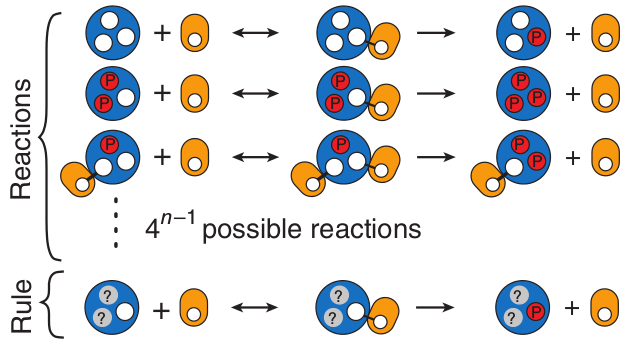
\includegraphics[scale=0.35]{pics/reaction_vs_rule.png}
\end{center}

\begin{itemize}
	\item there exists several representatives (Kappa, BNGL, Chromar, etc.)
	\begin{itemize}
		\item focused on detailed description instead of usability by the user 
	\end{itemize}
\end{itemize}

\end{frame}

% --------------------------------------------------------

\begin{frame}[fragile]{E-cyanobacterium.org}

\begin{itemize}
	\item an instance of Comprehensive Modelling Platform
	\item provide a tool for complete description and analysis of cyanobacteria ($\mathtt{CMSB`16}$)
	\item part of the project -- description of cyanobacteria metabolism and other processes
	\begin{itemize}
		\item naturally evolved language by biologists
	\end{itemize}
	\item in $\mathtt{SASB`16}$ introduced first version of the language with emphasis on annotation
\end{itemize}

\end{frame}

% --------------------------------------------------------

\begin{frame}[fragile]{BioChemical Space Language (BCSL)}

\begin{itemize}
	\item a rule-based language tailored for high-level abstraction of biochemical objects
	\item focus on human-readable syntax while preserving formal aspects needed for analysis
	\item part of an annotation format for Comprehensive Modelling Platform
\end{itemize}

\begin{center}
\hspace*{-0.7cm}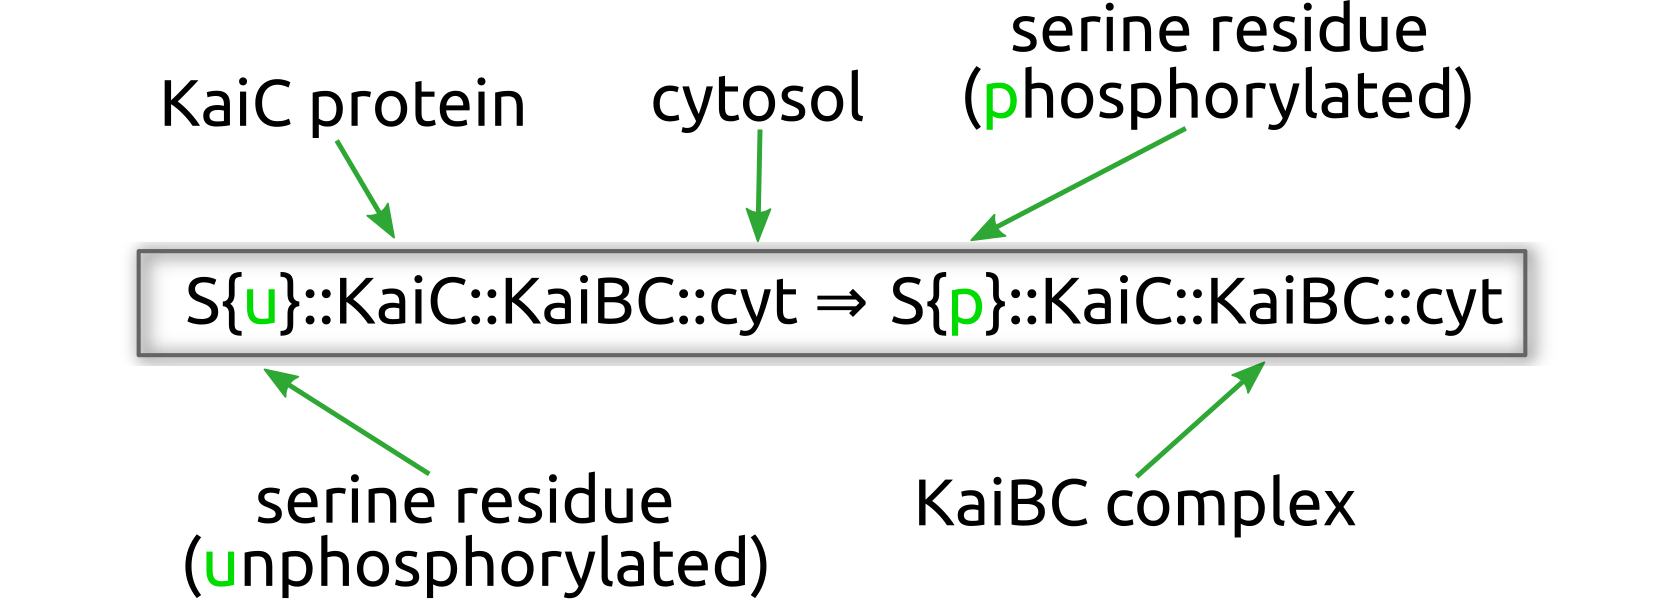
\includegraphics[scale=0.45]{pics/equation.png}
\end{center}

\end{frame}

% --------------------------------------------------------

\begin{frame}[fragile]{Analysis of rule-based models}

\begin{itemize}
	\item having a compact description, we want to use it in analysis process
	\begin{itemize}
		\item different mathematical models can be obtained for a given model, \\but we loose the compact description
		\item employ symbolic approach and static analysis
	\end{itemize}
\end{itemize}

\begin{minipage}{0.5\textwidth}
\begin{itemize}
	\item the problem of \\combinatorial explosion
\end{itemize}
\end{minipage}
\hfill
\begin{minipage}{0.4\textwidth}
\begin{center}
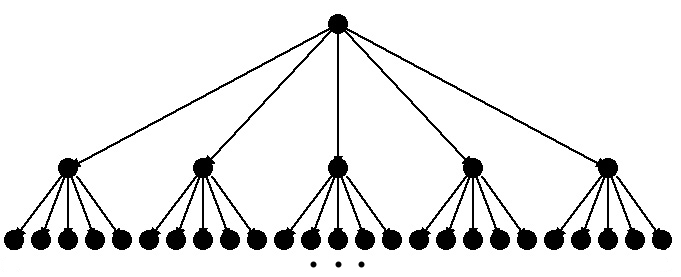
\includegraphics[scale=0.15]{pics/explosion}
\end{center}
\end{minipage}

\begin{itemize}
	
	\item analysis methods: simulation, model checking, parameter synthesis, robustness analysis

	\begin{itemize}
		\item provide answers to the most usual question in Systems biology
	\end{itemize}
\end{itemize}

\end{frame}

% --------------------------------------------------------

\begin{frame}[fragile]{Aims of the thesis}

\begin{enumerate}
	\item[I.] Analysis methods for rule-based formalisms

	\begin{itemize}
		\item general for rule-based approach
		\item efficient methods based on symbolic or static methods
		\item solve model checking, parameter synthesis, robustness analysis in particular
	\end{itemize}

	\item[II.] Software tool

	\begin{itemize}
		\item apply the developed methods to BCSL
		\item software support for maintenance and analysis of models in BCSL
	\end{itemize}
\end{enumerate}

\end{frame}

% --------------------------------------------------------

\begin{frame}[fragile]{Achieved results}

\begin{itemize}
	\item development of Comprehensive Modelling Platform with an application on cyanobacteria processes ($\mathtt{CMSB`16}$)
	\item first version of BCSL with emphasis on annotation ($\mathtt{SASB`16}$)
	\item most recent version of BCSL ($\mathtt{SASB`18}$) with several static analyses
	\item BCSgen software tool in Dean’s Program ($\mathtt{MUNI33/092015}$ and $\mathtt{MUNI33/062017}$)
\end{itemize}

\end{frame}

% --------------------------------------------------------

\begin{frame}[fragile]{Progression schedule}

Plan for future study and research activities:

\begin{itemize}
\item $\mathtt{Fall`19 ~-~ Fall`20}$: Development of analysis methods.
\item $\mathtt{Fall`20 ~-~ Spring`21}$: Implementation of developed methods.
\item $\mathtt{Spring`21}$: Release of a stable version of the software tool.
\item $\mathtt{Spring`21 ~-~ Fall`21}$: Work on the text of the PhD thesis.
\item $\mathtt{Fall`21}$: Thesis defence.
\end{itemize}

\end{frame}

% --------------------------------------------------------

\begin{frame}[fragile]{Summary}

\begin{itemize}
\item TBA
\end{itemize}

\end{frame}

\appendix

% --------------------------------------------------------

\backupbegin
\begin{frame}[fragile]{Analysis methods in particular}

{\small

\begin{itemize}
\item Given a rule-based model $\mu = (\mathcal{R}, \mathtt{M}_0)$ and a property formula $\phi$, the \textbf{problem of model checking} is to decide whether the model $\mu$ satisfies the property $\phi$.

\item Given a parametrised rule-based model $\mu = (\mathcal{R}, \mathtt{M}_0)$ and a formula $\phi$, the \textbf{problem of parameter synthesis} is to compute a partitioning of the given parameter space into three disjoint subsets: $\mathsf{TRUE}$ -- the parameter values satisfying the property, $\mathsf{FALSE}$ -- the parameter values violating the property, and $\mathsf{UNKNOWN}$ -- the result is not known.

\item The \textbf{problem of global robustness} of a model $\mu$ is defined as 

$$ R^{\mu}_{\phi, P} = \int_{P} \psi(p) D^{\mu}_{\phi}(p) dp $$

where $\phi$ is the property of the system under scrutiny, $P$ is the parameter space, $\psi(p)$ is the probability of the parametrisation $p$, and $D^{\mu}_{\phi}(p)$ is a local robustness.
\end{itemize}
}

\end{frame}
\backupend

% --------------------------------------------------------

\end{document}
